
\chapter{Prezentacja warstwy użytkowej projektu}
\label{chap:warstwa_uzytkowa}
W tym rozdziale przyjrzymy się aplikacji od strony użytkownika. Omówię kluczowe widoki i funkcje interfejsu graficznego (GUI) – od ekranu głównego, przez panele zakupowe, aż po moduły administratora.

\section{Ekran Główny i Proces Logowania}
Punktem startowym aplikacji jest ekran główny (\texttt{MainForm.java}), przedstawiony na Rys. \ref{fig:main_form}, który pełni rolę centrum nawigacyjnego. Z jego poziomu użytkownik może przejść do przeglądania listy produktów, rozpocząć proces zakupowy lub zalogować się do systemu. Panel logowania jest kluczowym elementem, który na podstawie wprowadzonych danych uwierzytelnia użytkownika i kieruje go do odpowiedniego modułu aplikacji. Zaimplementowano również funkcjonalność resetowania hasła, która po weryfikacji tożsamości użytkownika pozwala na ustawienie nowego hasła.

\begin{figure}[H]
    \centering
    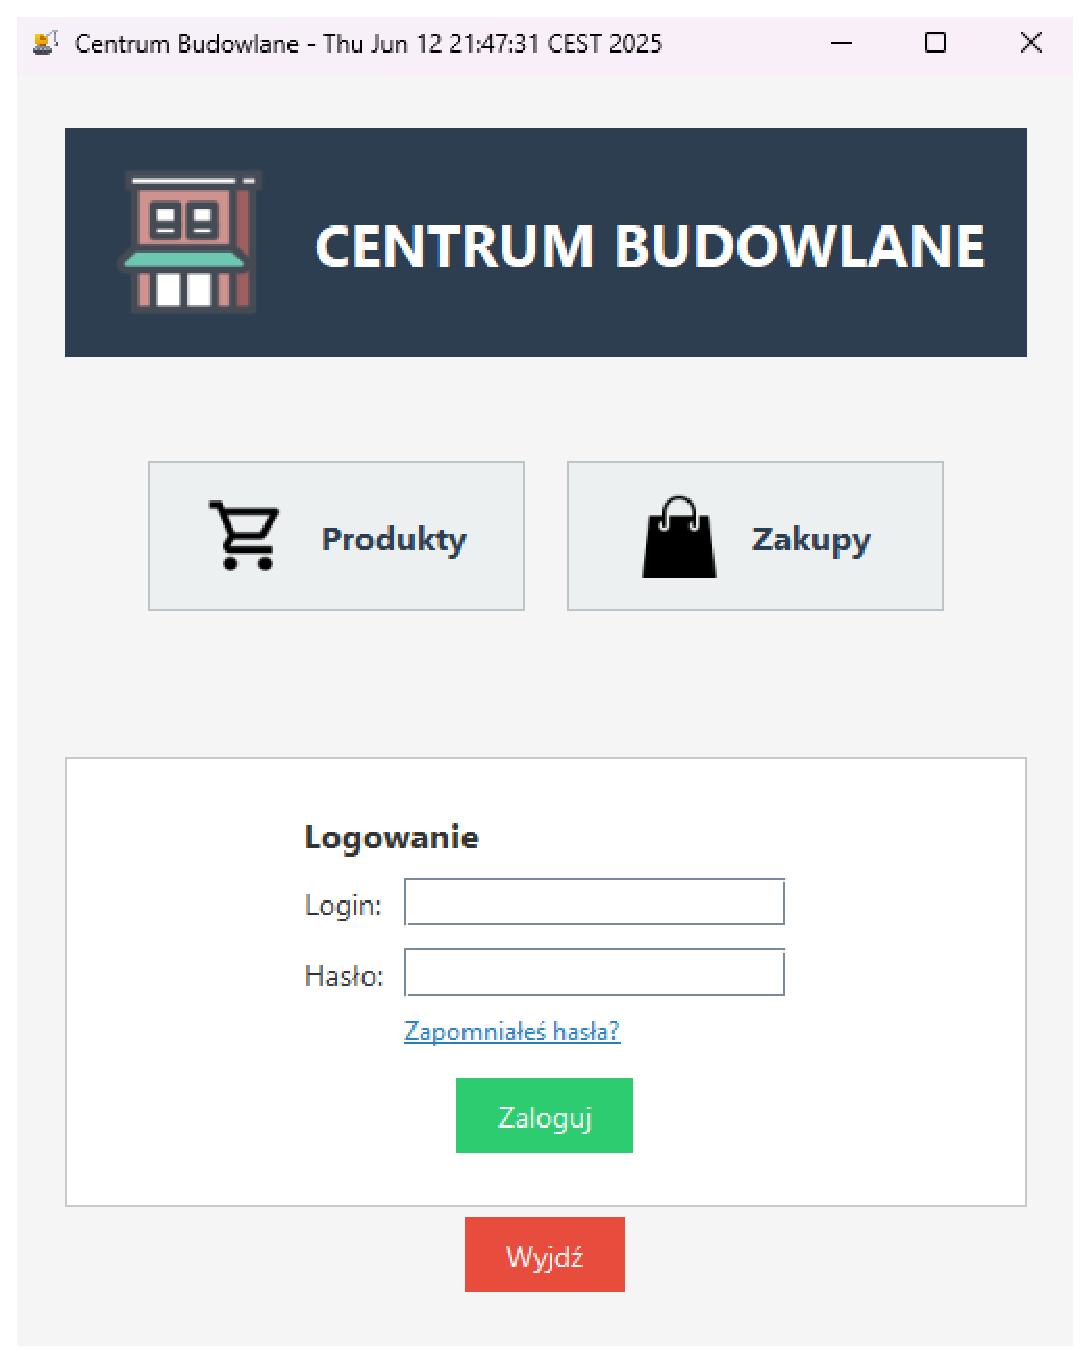
\includegraphics[width=0.6\linewidth]{figures/fig_0010.eps} 
    \caption{Główny ekran aplikacji z widocznym panelem logowania.}
    \label{fig:main_form}
    \small{Źródło: Opracowanie własne}
\end{figure}
\clearpage

\section{Interfejs Klienta}
Interfejs przeznaczony dla klienta został zaprojektowany z myślą o intuicyjności i wygodzie procesu zakupowego. Mimo że logika biznesowa i wygląd paneli dla klienta detalicznego (\texttt{ShopRetailForm.java}) i hurtowego (\texttt{ShopWholeSaleForm.java}) są do siebie bardzo zbliżone, istnieją między nimi kluczowe różnice.

\subsection{Panel Klienta Detalicznego}
Główny widok sklepu dla klienta detalicznego (Rys. \ref{fig:shop_retail}) składa się z trzech głównych sekcji: panelu danych klienta, listy dostępnych produktów oraz panelu koszyka. Klient może swobodnie przeglądać produkty, dodawać je do koszyka za pomocą przycisku i dedykowanego pola `JSpinner` do określania ilości , a następnie sfinalizować zamówienie. Kluczową cechą tego modułu jest to, że klient nie musi posiadać konta w systemie. Dane do wysyłki podawane są jednorazowo w oknie dialogowym `AddEditRetailCustomer`, które jest wywoływane przed złożeniem zamówienia.

\begin{figure}[H]
    \centering
    \includegraphics[width=0.85\linewidth]{figures/fig_0002.eps}
    \caption{Widok panelu zakupowego dla klienta detalicznego.}
    \label{fig:shop_retail}
    \small{Źródło: Opracowanie własne}
\end{figure}

\clearpage

\subsection{Panel Klienta Hurtowego}
Panel klienta hurtowego (\texttt{ShopWholeSaleForm.java}) jest wizualnie niemal identyczny z panelem detalicznym, jednak dostosowany do specyfiki klienta biznesowego. Główne różnice to:
\begin{itemize}
    \item \textbf{Ceny hurtowe:} Tabela produktów automatycznie ładuje niższe ceny hurtowe pobierane z bazy danych.
    \item \textbf{Stałe dane klienta:} Dane klienta, takie jak nazwa firmy czy NIP, są ładowane automatycznie po zalogowaniu i wyświetlane w górnej części panelu, co eliminuje potrzebę ich każdorazowego wprowadzania. Klient ma możliwość edycji swoich danych oraz zmiany hasła.
    \item \textbf{Warunki zamówienia:} System waliduje, czy zamówienie hurtowe spełnia minimalne progi, takie jak łączna liczba produktów w koszyku (minimum 3) oraz minimalna wartość zamówienia (50 zł).
\end{itemize}

\section{Panel Administratora}
Panel administratora (\texttt{AdminForm.java}) stanowi centrum dowodzenia aplikacją. Jest to główny pulpit, z którego administrator ma bezpośredni dostęp do wszystkich kluczowych modułów zarządczych. Został zaprojektowany w sposób modułowy, aby zapewnić szybki i intuicyjny dostęp do poszczególnych funkcjonalności. W centralnej części panelu wyświetlana jest tabela z listą ostatnich transakcji, co pozwala na bieżące monitorowanie aktywności w sklepie.

\begin{figure}[H]
    \centering
    \includegraphics[width=0.85\linewidth]{figures/fig_0011.eps}
    \caption{Główny widok panelu administratora.}
    \label{fig:admin_form}
    \small{Źródło: Opracowanie własne}
\end{figure}

Główne moduły, dostępne za pomocą dedykowanych przycisków, to:
\begin{itemize}
    \item \textbf{Zarządzanie Klientami} (\texttt{CustomerList.java})
    \item \textbf{Zarządzanie Magazynem} (\texttt{WarehouseForm.java})
    \item \textbf{Zarządzanie Transakcjami} (\texttt{ManagementTransactionForm.java})
\end{itemize}
Poniżej opisano szczegółowo działanie każdego z tych modułów.

\subsection{Zarządzanie Klientami i ich szczegóły}
Moduł \texttt{CustomerList.java} pozwala na przeglądanie, dodawanie (tylko hurtowych), edytowanie oraz usuwanie klientów. Za pomocą przełączników `JRadioButton` administrator może płynnie przełączać się między listą klientów detalicznych a hurtowych, a dane w tabeli są dynamicznie odświeżane.

Kluczową funkcjonalnością tego panelu jest możliwość wglądu w szczegółowe dane klienta po naciśnięciu przycisku "Szczegóły". Otwiera to nowe okno (\texttt{CustomerDetails.java}), które prezentuje kompleksowe informacje na temat wybranego klienta w trzech osobnych zakładkach:
\begin{itemize}
    \item \textbf{Informacje ogólne:} Wyświetlane są tu podstawowe dane, takie jak imię i nazwisko, typ klienta (detaliczny/hurtowy), łączna suma zakupów, adres oraz dane kontaktowe (telefon, e-mail, a w przypadku klienta hurtowego również NIP i nazwa firmy).
    \item \textbf{Historia transakcji:} Tabela zawierająca listę wszystkich transakcji dokonanych przez danego klienta, wraz z datą, kwotą, typem i listą zakupionych produktów.
    \item \textbf{Statystyki produktów:} Tabela grupująca wszystkie produkty zakupione przez klienta, przedstawiająca sumaryczną ilość oraz łączną wartość dla każdego z nich.
\end{itemize}

\begin{figure}[H]
    \centering
    \includegraphics[width=0.8\linewidth]{figures/fig_0012.eps}
    \caption{Panel szczegółowych informacji o kliencie.}
    \label{fig:customer_details}
    \small{Źródło: Opracowanie własne}
\end{figure}
\clearpage

\subsection{Zarządzanie Magazynem}
Widok magazynu (\texttt{WarehouseForm.java}) jest interfejsem bardzo zbliżonym wizualnie do panelu zarządzania klientami, jednak w pełni dostosowanym do operacji na produktach. Udostępnia narzędzia do pełnej kontroli nad asortymentem, pozwalając administratorowi na przeglądanie stanów magazynowych, sortowanie i filtrowanie danych (np. wyświetlając tylko produkty, których ilość jest niska), a także edytowanie ilości sztuk danego produktu. Zaimplementowano tu również funkcję składania zamówień do dostawców (\texttt{createWarehouseOrder}) oraz generowania raportów o niskich stanach magazynowych w formacie CSV. W panelu wyświetlane jest także aktualne saldo finansowe sklepu, które jest modyfikowane przy każdym zamówieniu magazynowym.

\subsection{Zarządzanie Transakcjami}
Ostatni moduł, \texttt{ManagementTransactionForm.java}, służy do przeglądania i analizy wszystkich transakcji w systemie. Administrator może filtrować transakcje według typu (detaliczne, hurtowe) oraz zakresu dat, korzystając z zintegrowanego komponentu kalendarza \texttt{LGoodDatePicker} \cite{LGoodDatePicker}. Po wybraniu transakcji z tabeli, w dedykowanym panelu wyświetlane są jej szczegółowe dane, w tym lista zakupionych produktów. Panel ten umożliwia również generowanie raportów CSV z przefiltrowanych danych.

\begin{figure}[H]
    \centering
    \includegraphics[width=0.85\linewidth]{figures/fig_0007.eps}
    \caption{Widok panelu zarządzania transakcjami z zintegrowanym kalendarzem.}
    \label{fig:management_transaction}
    \small{Źródło: Opracowanie własne}
\end{figure}
\clearpage
